\chapter{Results}
\label{chap:results}
%Link to audio examples (ok)
In this chapter, I compare the results of the experiments listed in Section \ref{sec:experiments-autotune}. I first examine the outputs on artificially de-tuned test data, and then on real-world karaoke examples from the MIR-1K dataset \cite{hsu2009improvement}. Based on histograms of the pitch deviations of the different outputs and their comparisons to the ground-truth Intonation dataset distribution, I choose one configuration. I use this configuration for an informal subjective listening test. Audio examples are publicly available\footnote{\href{https://adding-this-link}}.

%Synthesized set
\section{Experiments on the synthesized test set}

The validation loss curves for each experimental configuration are displayed in Figure \ref{fig:losses_plots}. For readability, the MSE is converted to absolute cents. The first three configurations did not use the song-level GRU extension, while the remaining three did. The last two configurations have different loss curves from the others because they were initialized using pre-trained weights. The initial large loss in these was due to the randomly initialized layers in the extension. One should note that the losses for different configurations are usually not comparable: the way the notes boundaries are assigned and the de-tuning techniques will all affect the value. How does error in cents correspond to musical accuracy? For perspective, 20 cents is the margin of error for some pitch detection algorithms \cite{kim2018crepe}. For intonation purposes, I think that 20 cents can sound out of tune, but starts to be acceptably close. An average error of 20 cents, which would include large errors, where the model corrected in the wrong direction, would be a highly accurate result. Even 30 cents could be considered a decent result for the same reason. 

The first two models trained for a longer time than the rest. When I tested them on real-world data, I was not happy with the audio result, and decided to test the other models at an earlier stage in training. Test results for the third model, which was trained on 223,000 songs instead of up to 498,000 songs, turned out to produce superior results. In later sections, I describe how I determined this in a more objective manner. What is striking is that the validation loss in all curves has not converged. Additionally, some models reached very small MSE values. For example, the ``HMM-HMM'' model, which used HMMs both to assign note boundaries and for de-tuning, reached 0.03, which corresponds to 17 cents average error. In practice, though, models that reached the lowest validation loss did not produce the best results on real-world data. I hypothesize that the models became too specialized for their specific configurations. 

\begin{figure}[t]
    \centering
    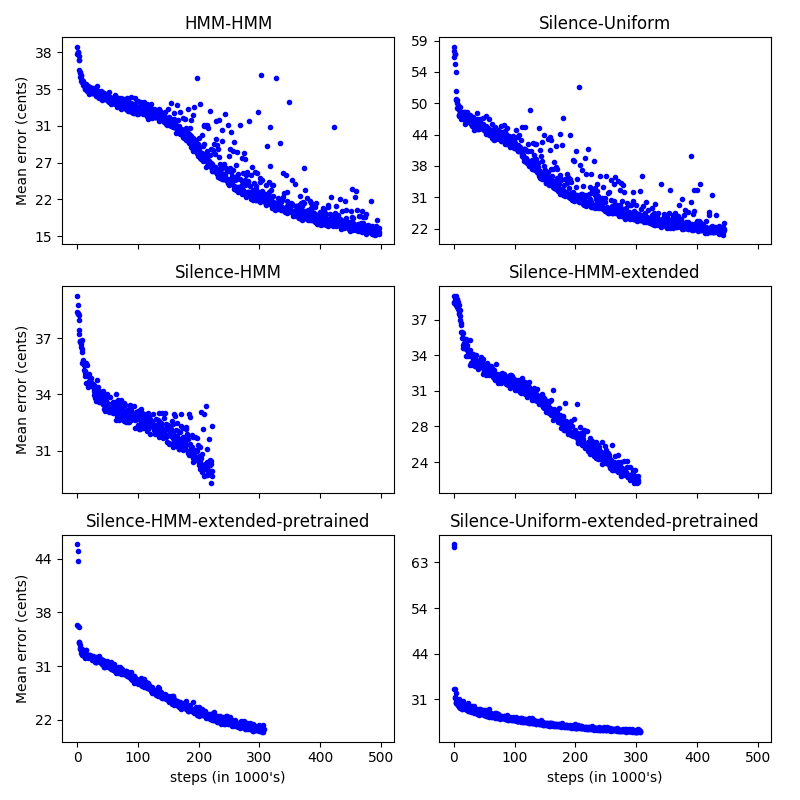
\includegraphics[width=\columnwidth]{figures/losses_plots.png}
    \caption{Validation losses for the respective configurations. The subtitle refers, first, to the note parsing technique, second, to the de-tuning technique, and then whether the model includes the song-level GRU extension layer and whether the model was initialized using pre-trained weights.}
    \label{fig:losses_plots}
\end{figure}

To compare the quality of the various configurations, I generated histograms of the pitch behavior in the results. These are displayed in Figures \ref{fig:test-comparison} and \ref{fig:mir-1k-comparison} for the synthesized test examples and the real-world MIR-1K dataset, respectively. The histograms show the pitch distributions before and after corrections. The pitch behavior is measured by generating the HMM described in Section \ref{sec:notes} to assign an equal-tempered scale degree to each frame of audio. I then measured the signed difference in cents between the equal-tempered scale degree and pYIN frequencies assigned to each frame. A wider histogram would indicate that more frames of audio are centered at pitches far from any equal-tempered scale degree. While this metric is arbitrary, it allows for comparison between different datasets.

In order to interpret these histograms, I also compared them to histograms of the input data, which consisted either of de-tuned data or of the MIR-1K dataset, histograms from the Intonation dataset ground truth, and those from professional performances from a separate dataset, DSD-100 \cite{SiSEC16}. These are displayed in Figure \ref{fig:dataset-comparison}. In Figure \ref{fig:test-comparison}, we see that the input data de-tuned using a random uniform distribution was more spread than the data de-tuned using the HMM. The output histogram that stands out is the third one, ``Silence-HMM'', which is more symmetric than the others and less spread. The same configuration produces the least spread results in Figure \ref{fig:mir-1k-comparison}. The reference datasets in Figure \ref{fig:dataset-comparison} show that the Intonation ground truth has a distribution similar to the output of the ``Silence-HMM'' model. This result made me choose the ``Silence-HMM'' model for the subjective listening test.

Figure \ref{fig:dataset-comparison} also displays the limitations of using the Intonation dataset as ground truth. The professional-level DSD-100 dataset has a narrower spread than the Intonation dataset, showing how different the pitch distribution is between amateur singers selected for accurate pitch, and professionals. The ``Silence-HMM'' model is able to shift the pitch deviation distribution of both synthesized and real-world data so that its corrected distribution matches that of the ground truth. Without professional-level data, though, it will not produce an outcome that has a distribution like the DSD-100 dataset.

\begin{figure}[t]
    \centering
    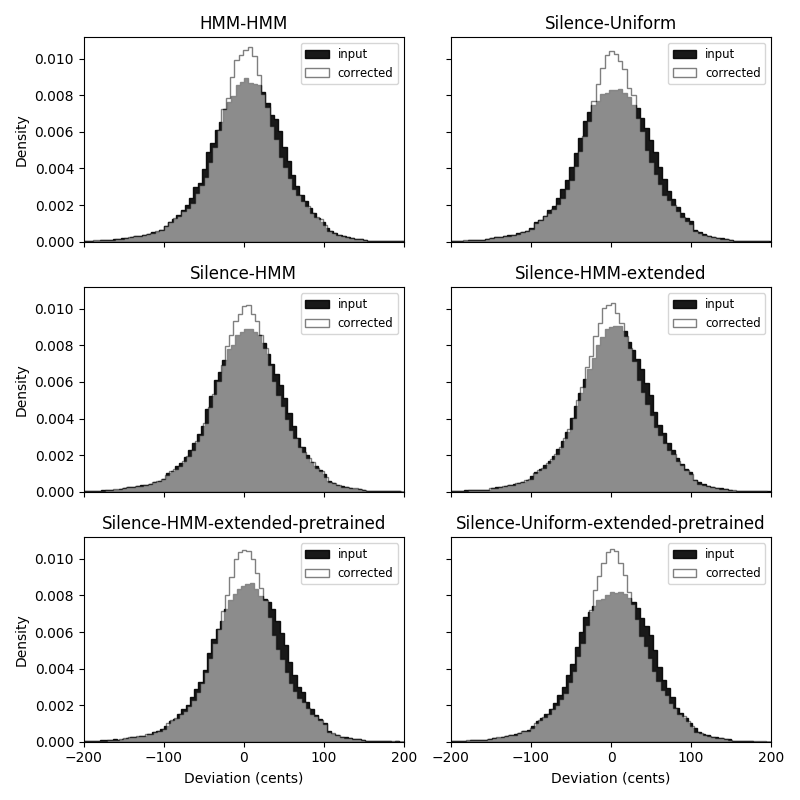
\includegraphics[width=\columnwidth]{figures/test-comparison.png}
    \caption{Pitch deviation histograms of the synthesized test data before and after corrections. Input data de-tuned using a random uniform distribution was more spread than the data de-tuned using the HMM. The third output histogram, ``Silence-HMM'' stands out as being the most symmetric.}
    \label{fig:test-comparison}
\end{figure}

\begin{figure}[t]
    \centering
    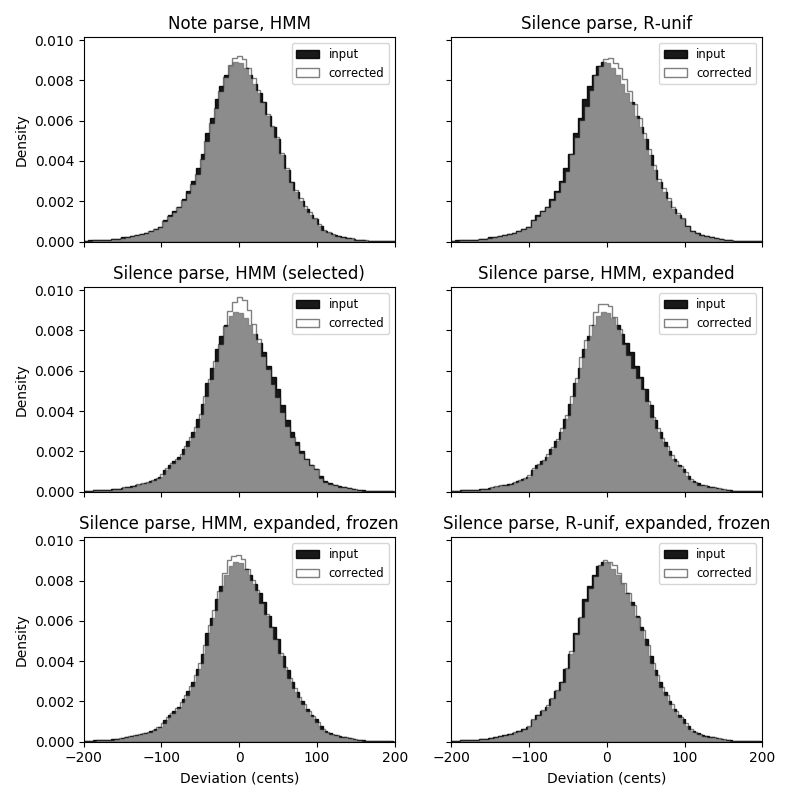
\includegraphics[width=\columnwidth]{figures/mir-1k-comparison.png}
    \caption{Pitch deviation histograms of the real-world MIR-1K data before and after corrections. The third output histogram, ``Silence-HMM'', again stands out as being the most symmetric.}
    \label{fig:mir-1k-comparison}
\end{figure}

\begin{figure}[t]
    \centering
    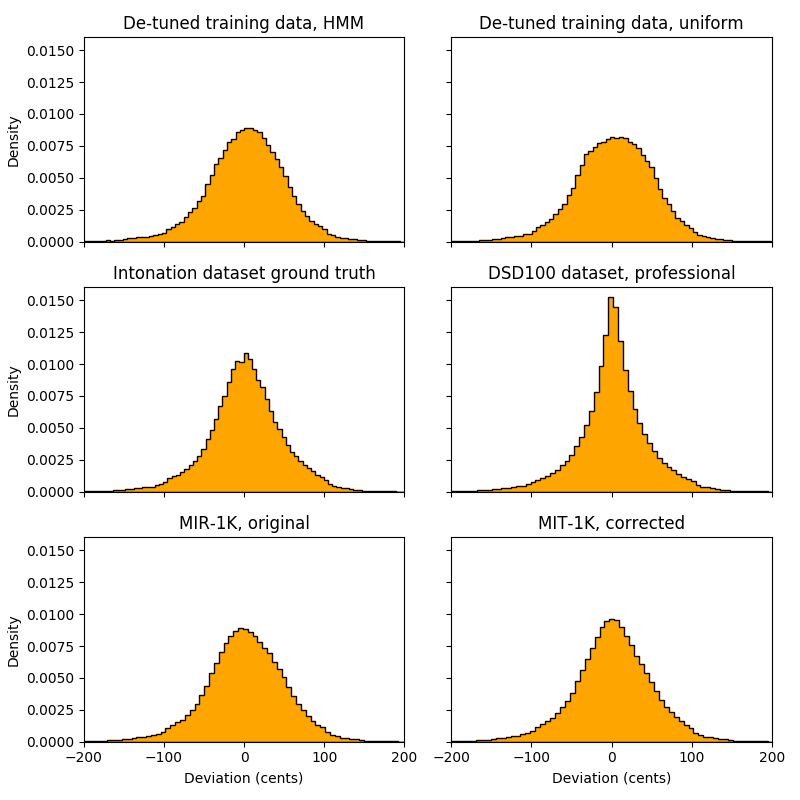
\includegraphics[width=\columnwidth]{figures/dataset-comparison.png}
    \caption{Pitch deviation histograms of various datasets. The first row displays artificially de-tuned training data. Note that it appears quite similar to the MIR-1K real-world data before corretions, shown in the bottom left subplot. The left subplot in the middle row shows the distribution of the Intonation ground truth. This resembles the histogram of the MIR-1K data after corrections using the ``Silence-HMM'' model, shown in the bottom right subplot. The middle-right subplot shows the distribution of a small, professional dataset. It looks strikingly different from the rest.}
    \label{fig:dataset-comparison}
\end{figure}



%- Loss curves
%- Analysis
%Subjective listening test
\section{Subjective listening test}
\label{sec:subjective-test}
%- Listening test setup
I conducted a subjective listening test to qualitatively assess the pitch correction algorithm's performance. I selected ten twenty-second samples from the MIR-1K original dataset, which I considered musically interesting. I had not heard the pitch correction results in these performances before when selecting the samples. I chose twenty seconds because this sample length gave listeners an idea of how the algorithm performed on a full musical phrase. Any ambiguity due to the sample length could be resolved by adding a comment. Table \ref{table:audio-samples} shows the samples along with their musical characteristics and why I chose them. 

\begin{table*}
\centering
\begin{tabularx}{\columnwidth}{ |c|c|X| } 
\hline
\multicolumn{3}{|c|}{\textbf{Subjective test samples from MIR-1K}}\\
\hline\hline
\textbf{Sample name} & \textbf{Start second} & \textbf{Description} \\
\hline\hline
Ariel 1 & 0 & Mostly close to an accurate pitch; A couple notes are off by a larger amount, and one by a semitone \\
\hline
Ariel 2 & 23 & Mostly slightly off, sometimes up to 50 cents off\\ 
\hline
Annar 4 & 3 & In tune\\ 
\hline
Amy 7 & 27 & An audible MIDI drone is playing the melody\\
\hline
Davidson 4 & 6 & Very low voice, mostly close but slightly off pitch \\ 
\hline
Bobon 4 & 2 & Melody has some very long notes; Pitch is often off, sometimes by more than 40 cents\\ 
\hline
Geniusturtle 4 & 9 & One note is over 50 cents off, many jumps in the melody, one section is legato\\ 
\hline
Stool 4 & 0 & Mildly off overall; the tempo is on the faster side; the melody has jumps; there is an audible MIDI drone\\ 
\hline
Fdps 4 & 17 & Slow tempo, jumps in the melody, a couple notes are off by more than 50 cents\\ 
\hline
Jmzen 4 & 0 & Very far off overall\\ 
\hline
\end{tabularx}
\label{table:audio-samples}
\caption{Description of the audio samples from MIR-1K used for the subjective listening test, and their diverse characteristics that test the program under varying conditions}
\end{table*}

The question arises of whether a simple pitch correction technique could achieve comparable or superior results with significantly less time and resources. I generated a baseline algorithm for this reason. The baseline retains many the characteristics of the proposed model: it shifts each note by a constant to retain a natural sound, and assigns note boundaries where the pYIN pitch detection algorithm assigned silence. Its pitch corrections, however, are based on the equal-tempered scale. For each note, it computes the median pitch from the pYIN---which should be the longest note's median in legato sections treated as a single note. It then shifts the note so that its new median is the nearest equal-tempered scale degree. Figure \ref{fig:baseline_tuning} shows the behavior of the baseline algorithm.

\begin{figure}[t]
    \centering
    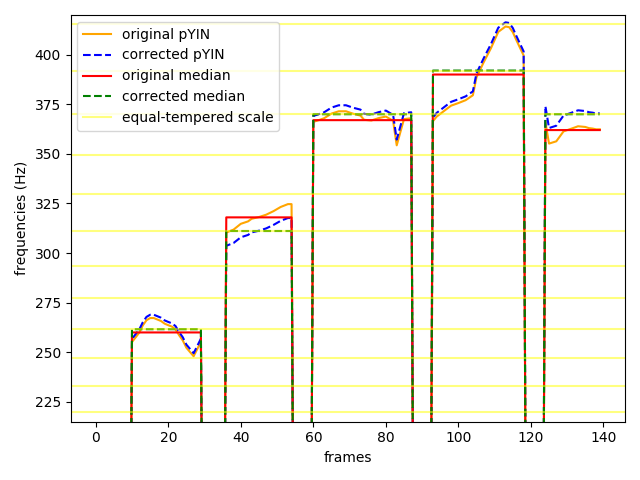
\includegraphics[width=\columnwidth]{figures/baseline_tuning.png}
    \caption{Example of the baseline system's corrections. The system determines note boundaries in the same way as the selected model, assigning them where silence occurs. It computes the median of each note, and shifts it so that its new median is the nearest equal-tempered scale degree.}
    \label{fig:baseline_tuning}
\end{figure}

For both algorithms, the pitch shifts applied to the audio were computed using TD-PSOLA. The only difference between the outputs is the amount of shift. In a subjective test conducted in previous work, \cite{wager2020deep}, listeners were asked to select when comparing the original audio to the corrected audio which version sounded more natural. Listeners did not hear a difference between samples, which indicates that TD-PSOLA doesn't produce a significant amount of artifacts that would make it difficult to rate the quality of the system only based on musical intonation instead of audio quality.

Each listener was assigned four samples: two pairs comparing the baseline outputs to the original, and two comparing the corrected outputs to the original using the ``Silence-HMM'' model. The listeners did not know which algorithms were used in each pair. They were asked to indicate which performance they considered more accurate in terms of pitch, and could optionally leave comments. Table \ref{table:audio-samples-results} shows the results and anonymized comments. A total of N participants provided M responses. From the results, we can see that ...

\begin{table}
  \begin{center}
    \caption{Baseline versus original}
    \label{tab:table1}
    \begin{tabularx}{\columnwidth}{|l|l|X|}
    \hline
\textbf{Sample name} & \textbf{Score} & \textbf{Comments} \\
\hline\hline
Ariel 1 & 0-2 & "Not easy to hear the difference"; "Difficult. Notes at 6 and 16 seconds are out of tune in both samples. Note between 9 and 11 might be better in original. Original is better, neither is great."\\
\hline
Ariel 2 & 0-2 & "Both mostly in tune"; "Very close, both pretty much in tune"\\ 
\hline
Annar 4 & 1-0 & "Baseline is so out of tune that it is difficult to figure out what the melody is, but one can perhaps can make more sense of Original."\\ 
\hline
Amy 7 & 1-0 & - "Baseline gets a mild preference. The original gets an overall score of 9/10"\\
\hline
Davidson 4 & 0-0 & N/A\\ 
\hline
Bobon 4 & 0-2 & "Both are pretty bad, but original might be somewhat more in tune" \\ 
\hline
Geniusturtle 4 & 1-0 & N/A\\ 
\hline
Stool 4 & 0-1 & "Strong preference for original, the baseline gets score 7/10"\\ 
\hline
Fdps 4 & 0-0 & "both moderately out of tune - one's ear's might be getting a bit tired at this point"; "original sounded clearly more in tune, starting from a pretty weak base in baseline\\ 
\hline
Jmzen 4 & 1-1 & "both are moderately out of tune, also the singer might not always hit the right note; now one's ears might be too tired"; "Very close, original is better e.g., on second 7" \\ 
\hline
    \end{tabularx}
  \end{center}
\end{table}

\begin{table}
  \begin{center}
    \caption{Corrected versus original}
    \label{tab:table1}
    \begin{tabularx}{\columnwidth}{|l|l|X|}
    \hline
\textbf{Sample name} & \textbf{Score} & \textbf{Comments} \\
\hline\hline
Ariel 1 & 0-1 & N/A \\
\hline
Ariel 2 & 0-0 & N/A \\ 
\hline
Annar 4 & 0-0 & N/A \\ 
\hline
Amy 7 & 0-0 & N/A \\
\hline
Davidson 4 & 3-0 & "Both are very accurate, very difficult to tell the difference"; "Both are pretty much in tune, a note at second 5 might be better in corrected"; "Strong preference for corrected, worse signal gets overall score 9/10"\\ 
\hline
Bobon 4 & 1-0 & N/A \\ 
\hline
Geniusturtle 4 & 3-0 & "Corrected is clearly better"; "Corrected sounded clearly more in tune"; "Corrected is slightly better, original gets score 6/10"\\ 
\hline
Stool 4 & 2-0 & "Corrected is clearly better"; "Notes at seconds 4 and 9 are better in corrected" \\ 
\hline
Fdps 4 & 1-1 & both moderately out of tune - one's ear's might be getting a bit tired at this point \\ 
\hline
Jmzen 4 & 0-0 & N/A \\ 
\hline
    \end{tabularx}
  \end{center}
\end{table}




%- Results
%\subsection{Results on the subjective listening test}
%\label{sec:subjective-results}
%Globally, in pairs where the subjects compared the proposed program to the original performance, they selected the proposed 33 times and the %original 35 times, for a success rate of 49\% with a one-sided binomial test p-value of 0.45. The baseline versus the original produced numbers 24 %and 34, or 41\% success rate with p-value 0.12. The proposed model versus the baseline produced 31 and 29, or a success rate of 52\% with p-value %0.45. These global numbers themselves do not suggest an advantage in using either pitch corrector. The number of responses is also quite small, which leaves uncertainty in these responses because not all versions of all 96 clips were covered and each clip is quite different. In future work, we plan to conduct a larger-scale subjective test.

%In our small sample, we found some patterns worth investigating once we conduct a larger test. One such pattern is that subjects might prefer proposed corrected signals when the quality of the original singing is slightly off key, but not too far. We identify such cases by looking at note-level pitch deviation statistics (in cents) between the original performance and the ground-truth MIDI score, generously provided by Smule, Inc. For example, we computed the standard deviation of the cents differences between the original singing and the ground-truth MIDI score. We found that the subjects usually favor a corrected example if the original was within a particular standard deviation range (between 40 and 60 cents). 19 out of 24, or 79\% of the preferred corrected examples were in this range, compared to only 16\% (3 out of 19) preferred original examples. While we would need more data for reliable results, we expect this behavior due to the imperfectly tuned nature of our crowdsourced training data used as in-tune ground truth---only some noticeable amount of off-pitch can be fixed by the trained model. Meanwhile, the model is exposed only to up to a semitone pitch shift, suggesting that too much variation in the test signal cannot be fixed, either. 

%We also compared the proposed method to the baseline. In 18 out of 21 or 86\% of performances where the proposed model was selected, the median of the absolute value of deviations in cents within two semitones was less than 46. However, 8 out of 20, or 40\% of performances where the baseline was selected were in the same range. This second result again that the proposed model might work better when performances are already relatively accurate. See Table \ref{tab:result-autotune} for a summary. 


%- Analysis

